\documentclass[10pt,letterpaper]{article}
\usepackage[spanish]{babel}
\usepackage{listings}
\usepackage{graphicx} %paqute para que pueda jalar mi imagen del diagrama
\usepackage{float}
% Preámbulo

\title{Análisis de ingeniería inversa sobre un sistema \textit{legacy}}
\author{Base de Datos }
\date{\today}

\usepackage{xcolor}

\definecolor{codegreen}{rgb}{0,0.6,0}
\definecolor{codegray}{rgb}{0.5,0.5,0.5}
\definecolor{codepurple}{rgb}{0.58,0,0.82}
\definecolor{backcolour}{rgb}{0.95,0.95,0.92}

\lstdefinestyle{mystyle}{
    backgroundcolor=\color{backcolour},   
    commentstyle=\color{codegreen},
    keywordstyle=\color{magenta},
    numberstyle=\tiny\color{codegray},
    stringstyle=\color{codepurple},
    basicstyle=\ttfamily\footnotesize,
    breakatwhitespace=false,         
    breaklines=true,                 
    captionpos=b,                    
    keepspaces=true,                 
    numbers=left,                    
    numbersep=5pt,                  
    showspaces=false,                
    showstringspaces=false,
    showtabs=false,                  
    tabsize=2
}
\lstset{style=mystyle}

 

\begin{document}
\maketitle




\section{Introducción}
Se nos ha encomendado realizar ingenria inversa y posteriormente el analisis de un conjunto de archivos que comprenden
la definicion estructural y logica de la Base de Datos de un sistema "Legacy".Con la finalidad de practicar e integrar todo lo 
aprendido 
\section{Descripción del problema}
Lo que hace este programa en SQL , es como un archivero digital para organizar los datos 
de una escuela,y que todo este donde debe de estar ya que crea diferentes listas que se
conectan entre si para guardar la informacion bien estructurada y limpia.
\section{Análisis}
Pero ,¿Qué es lo que hace exactamente ?
Bueno en primer lugar tenemos que crear un espacio inicial donde se va a guardar todo 
\begin{table}[h!]%para que lo ponga justo abajo de "Analisis"
    \begin{tabular}{| c |p{10cm} |} %esto srive para dar un salto de linea para que no se siga de largo LaTex
        \hline
        TABLAS & ¿QUE ORGANIZA? \\
        \hline
        Departamentos y Profesores & Hace una lista de las areas de la escuela
                                    y registra a los profesores identificando a que 
                                    area pertence cada uno\\ \hline
        
        Curos y Aulas              & Registra materias que se imparten , que profesor las imparte
                                     y los salones con disponibilidad y cupo maximo\\ \hline

        Horarios                   & Acomoda el día , a que hora y en que salón toca cada materia\\ \hline
        
        Estudiantes e Inscripciones & Guarda los datos personales de los alumnos y lleva un control de 
                                      las materias que tienen inscritas\\ \hline
        
        Calificaciones                & Crea un espacio exclusivo para guardar las calificaciones finales de los
                                      alumnos en cada materia que tomaron\\ \hline
    \end{tabular}
\end{table}

\section{Diagramas y resultados}
\begin{figure}[H]
    \includegraphics[scale=0.4]{images/Ingeneria-Inversa.png}
    \caption{Diagrama Entidad - Relacion del Sistema}
    \label{fig-Ingeneria-Inversa}
    \end {figure}
\section{Implementación y validación}
\begin{figure}[H]
 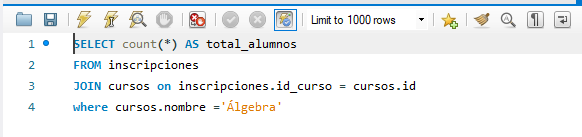
\includegraphics[width=\textwidth]{images/P1.png}
  \caption{Implementacion de Cosulta en SQL para la Pregunta 1}

\end{figure}
\begin{figure}[H]
    \includegraphics[scale=0.4]{images/Ingeneria-Inversa.png}
    \caption{Diagrama Entidad - Relacion del Sistema}
    \label{fig-Ingeneria-Inversa}
    \end {figure}
\section{Implementación y validación}
\begin{figure}[H]
 \graphicspath{{images/}}
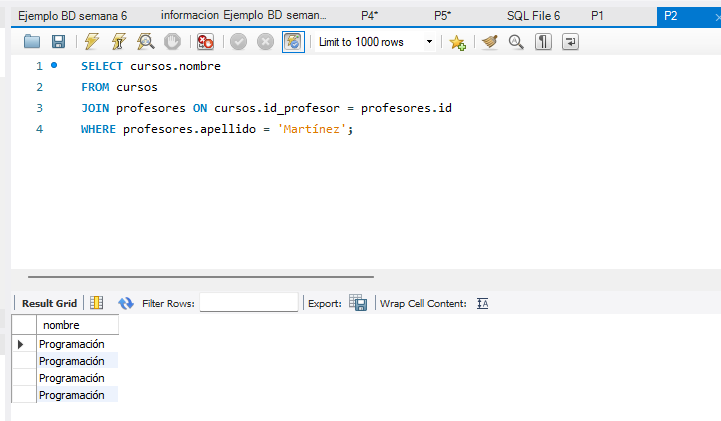
\includegraphics[width=\textwidth]{P2.png}
  \caption{Implementacion de Cosulta en SQL para la Pregunta 2}

\end{figure}


\section{Conclusiones}
 




\end{document}